%%%%%%%%%%%%%%%%%%%%%%%%%%%%%%%%%%%%%%%%%%  不使用 authblk 包制作标题  %%%%%%%%%%%%%%%%%%%%%%%%%%%%%%%%%%%%%%%%%%%%%%
%-------------------------------PPT Title-------------------------------------
\title{24-选讲专题:~计算材料数据库简介}
%-----------------------------------------------------------------------------
%----------------------------Author & Date------------------------------------

%\author[\textrm{Jun\_Jiang}]{姜\;\;骏\inst{}} %[]{} (optional, use only with lots of authors)
%% - Give the names in the same order as the appear in the paper.
%% - Use the \inst{?} command only if the authors have different
%%   affiliation.
%\institute[BCC]{\inst{}%
\institute[Gain~Strong]{\inst{}%
%\vskip -20pt 北京市计算中心}
\vskip -20pt {\large 格致斯创~科技}}
\date[\today] % (optional, should be abbreviation of conference name)
{%	{\fontsize{6.2pt}{4.2pt}\selectfont{\textcolor{blue}{E-mail:~}\url{jiangjun@bcc.ac.cn}}}
\vskip 45 pt {\fontsize{8.2pt}{6.2pt}\selectfont{%清华大学\;\;物理系% 报告地点
	\vskip 5 pt \textrm{2023.04.22}}}
}

%% - Either use conference name or its abbreviation
%% - Not really information to the audience, more for people (including
%%   yourself) who are reading the slides onlin%%   yourself) who are reading the slides onlin%%   yourself) who are reading the slides onlineee
%%%%%%%%%%%%%%%%%%%%%%%%%%%%%%%%%%%%%%%%%%%%%%%%%%%%%%%%%%%%%%%%%%%%%%%%%%%%%%%%%%%%%%%%%%%%%%%%%%%%%%%%%%%%%%%%%%%%%

\subject{}
% This is only inserted into the PDF information catalog. Can be left
% out.
%\maketitle
\frame
{
%	\frametitle{\fontsize{9.5pt}{5.2pt}\selectfont{\textcolor{orange}{“高通量并发式材料计算算法与软件”年度检查}}}
\titlepage
}
%-----------------------------------------------------------------------------

%------------------------------------------------------------------------------列出全文 outline ---------------------------------------------------------------------------------
%\section*{}
%\frame[allowframebreaks]
%{
%  \frametitle{Outline}
%%  \frametitle{\textcolor{mycolor}{\secname}}
%  \tableofcontents%[current,currentsection,currentsubsection]
%}
%%在每个section之前列出全部Outline
%%类似的在每个subsection之前列出全部Outline是\AtBeginSubsection[]
%\AtBeginSection[]
%{
%  \frame<handout:0>%[allowframebreaks]
%  {
%    \frametitle{Outline}
%%全部Outline中,本部分加亮
%    \tableofcontents[current,currentsection]
%  }
%}

%-----------------------------------------------PPT main Body------------------------------------------------------------------------------------
\small
%\section{\rm{VASP~}软件中\rm{PAW~}计算的实现}
%\frame
%
%	\frametitle{\textrm{VASP}计算的特色}
%	相比于与普通的第一原理计算软件,\textrm{VASP}很好地平衡了计算效率和精度的问题,总的来说,\textrm{VASP}主要通过这几个特色保证了计算的高效能
%	\begin{itemize}
%	     \item 迭代与优化算法的多样性\\
%		     本质上电荷密度迭代 \textrm{\&\&} 体系总能量优化是相同的优化问题,采用了类似的算法\upcite{CMS6-15_1996,PRB54-11169_1996}:\\
%			\textcolor{blue}{\textrm{Pseudo-Newton、Conjugate-Gradient、Broyden~mix、damping-factor、RMM-DIIS}}
%	     \item 尽可能采用局域基(原子轨道基)函数:~\\
%		     \textcolor{blue}{\textrm{LREAL}}=\textcolor{red}{\textrm{.TRUE.}}\\
%			优化的投影函数也尽可能在实空间表示
%	     \item \textrm{PAW}原子数据集:\textcolor{blue}{优异的赝势}\upcite{PRB59-1758_1999}
%	\end{itemize}
%}

\appendix
\frame
{
	\frametitle{向我国量子化学学科的奠基人致敬!}
\begin{figure}[h!]
	\centering
\centering
\vspace{-10.5pt}
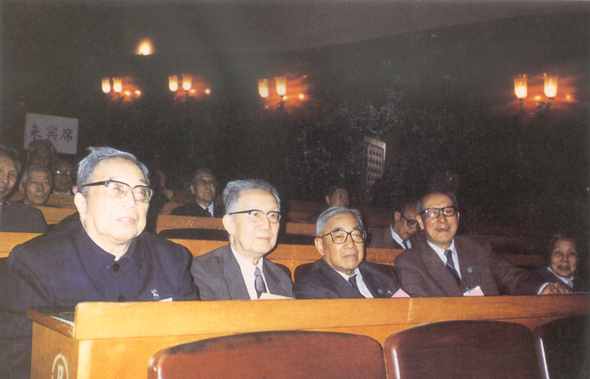
\includegraphics[height=0.58\textwidth,width=1.0\textwidth,viewport=0 0 435 250,clip]{Figures/1994_6_5.jpg}
\caption{\fontsize{6.8pt}{5.0pt}\selectfont{1994年6月5日~唐敖庆~教授(1915-2008)、吴征铠~教授(1913-2007)、卢嘉锡~教授(1915-2001)、徐光宪~教授(1920-2015)和高小霞~教授(1919-1998)(从左到右)在第七次院士大会上}}
%\caption{1994年6月5日\fbox{唐敖庆}教授、\fbox{吴征铠}教授、\fbox{卢嘉锡}教授、\fbox{徐光宪}教授和\fbox{高小霞}教授(从左到右)在第七次院士大会上}
%\caption{1994年6月5日\frame{唐敖庆}教授、\frame{吴征铠}教授、\frame{卢嘉锡}教授、\frame{徐光宪}教授和\frame{高小霞}教授(从左到右)在第七次院士大会上}
\label{Tang_Wu_Lu_Xu}
\end{figure}
}

\frame
{
	\frametitle{向我国固体物理学科的奠基人致敬!}
\begin{figure}[h!]
\centering
\vspace{-15.5pt}
\subfigure[\fontsize{7.2pt}{5.0pt}\selectfont{黄昆~教授(1919-2005)}]{
\label{fig:Huang}
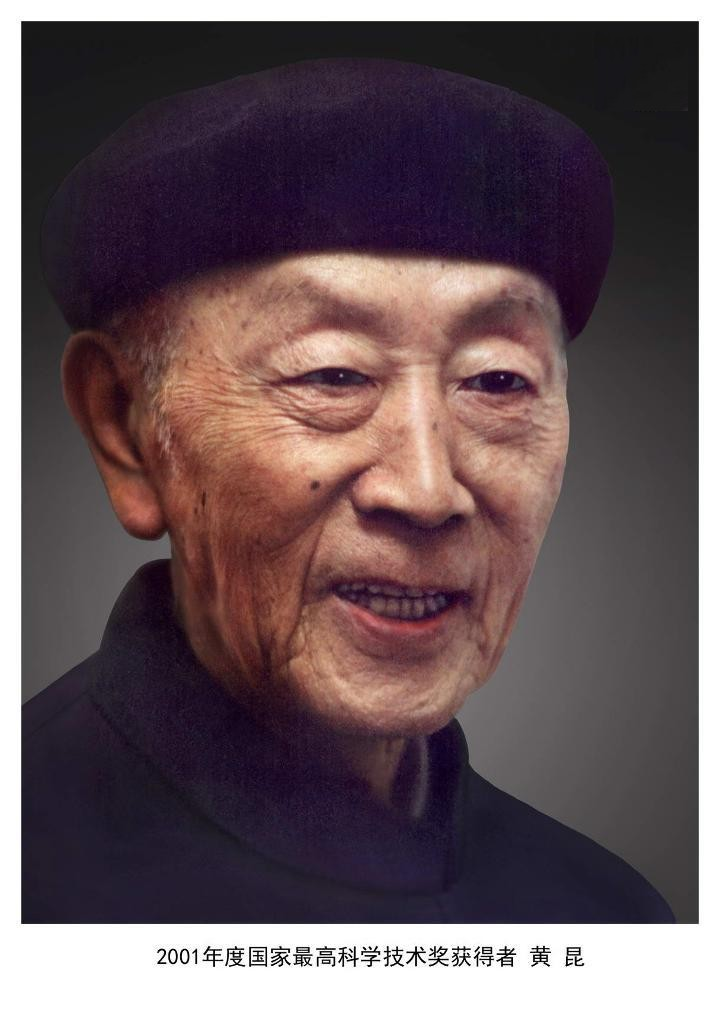
\includegraphics[height=1.20in,width=1.9in,viewport=-300 90 1020 1000,clip]{Figures/Huang.jpg}}
\subfigure[\fontsize{7.2pt}{5.0pt}\selectfont{谢希德~教授(1921-2000)}]{
\label{fig:Xie}
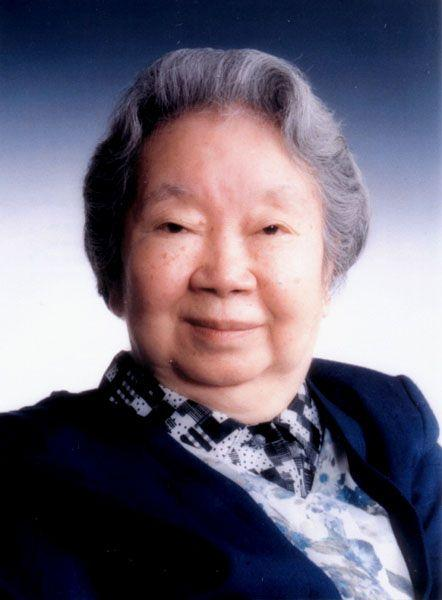
\includegraphics[height=1.20in,width=1.9in,viewport=-180 0 680 575,clip]{Figures/Xie.jpg}}
\subfigure[\fontsize{7.2pt}{5.0pt}\selectfont{彭桓武~研究员(1915-2007)}]{
\label{fig:Peng}
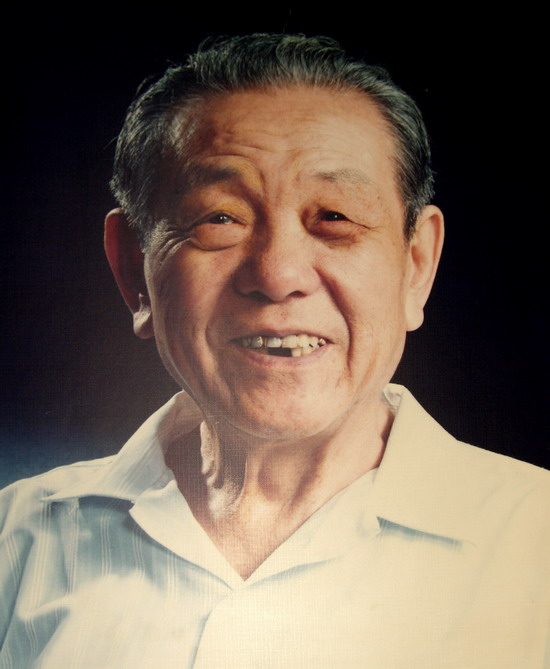
\includegraphics[height=1.20in,width=1.9in,viewport=-200 0 850 660,clip]{Figures/Peng.jpg}}
\subfigure[\fontsize{7.2pt}{5.0pt}\selectfont{程开甲~教授(1918-2018)}]{
\label{fig:Cheng}
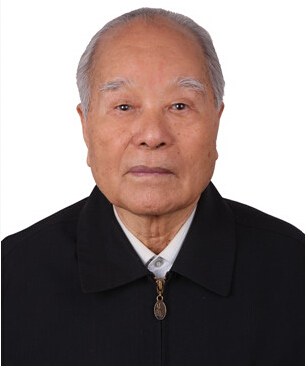
\includegraphics[height=1.20in,width=1.9in,viewport=-110 0 325 275,clip]{Figures/Cheng.jpg}}
%\caption{}%
\label{Peng_Huang_Xie_Cheng}
\end{figure}
}

\frame
{
\begin{figure}[h!]
\vskip -5pt
\centering
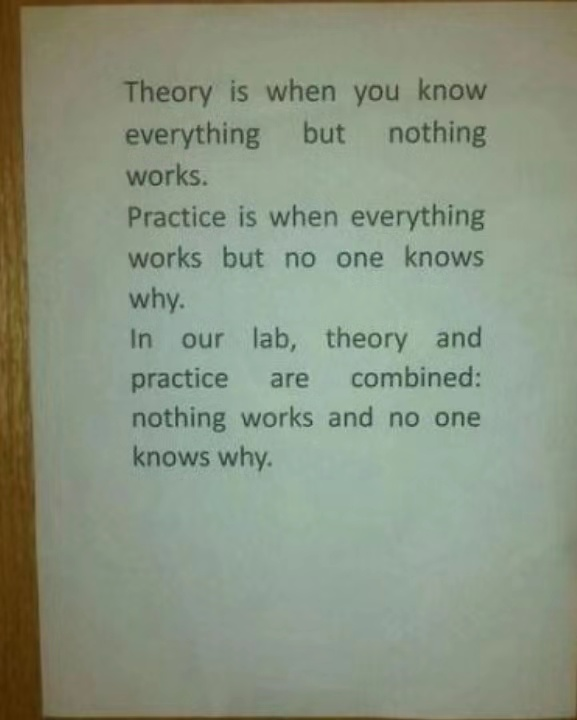
\includegraphics[height=2.8in,width=2.5in,viewport=110 225 505 660,clip]{Figures/Theory_Practice.jpg}
\label{Theory_Practice}
\end{figure}
}

\frame
{
	\frametitle{}
\begin{figure}[h!]
\centering
\vspace{-5.5pt}
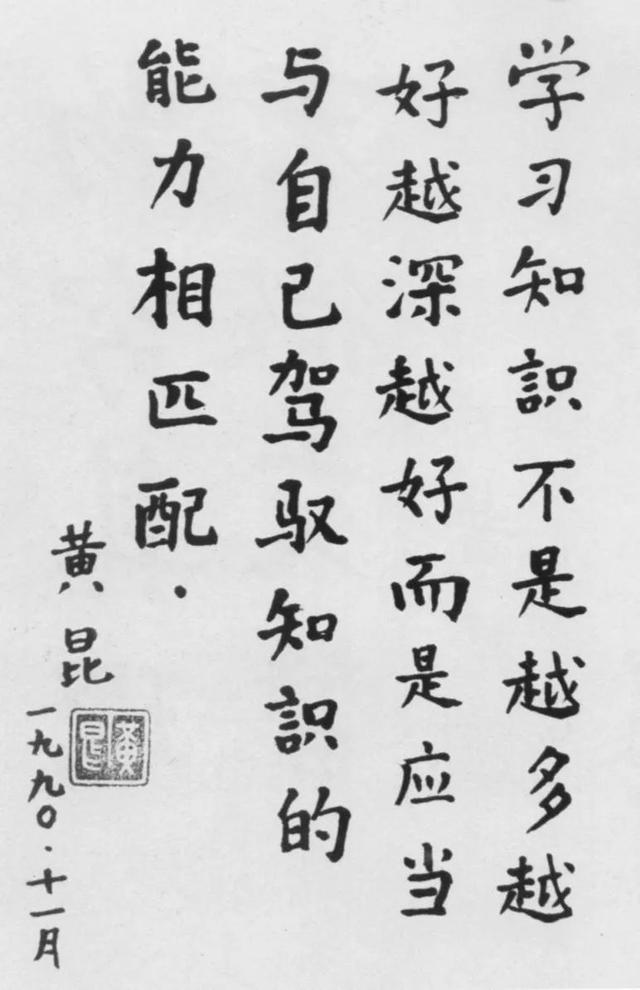
\includegraphics[height=0.65\textwidth]{Figures/Quote-Huang_Kun.jpg}
\caption{\fontsize{6.2pt}{5.2pt}\selectfont{黄昆~教授的治学名言}}
\label{Quote-Huang_Kun}
\end{figure}
}

%\frame
%{
%	\frametitle{卖油翁:~\textcolor{red}{无他~但手熟尔}}
%%陈康肃公尧咨善射,当世无双 ,公亦以此自矜。尝射于家圃,有卖油翁释担而立,睨之,久而不去。见其发矢十中八、九,但微颔之。康肃问曰:“汝亦知射乎?吾射不亦精乎?”翁曰:“无他,但手熟尔。”康肃忿然曰:“尔安敢轻吾射!”翁曰:“以我酌油知之。”乃取一葫芦置于地,以钱覆其口,徐以杓酌油沥之,自钱孔入而\footnote{一作“而入”}钱不湿。因曰:“\textcolor{red}{我亦无他,惟手熟尔}。”康肃笑而遣之。此与庄生所谓“解牛”、“斫轮”者何异?
%\begin{figure}[h!]
%\centering
%\vspace{-10.5pt}
%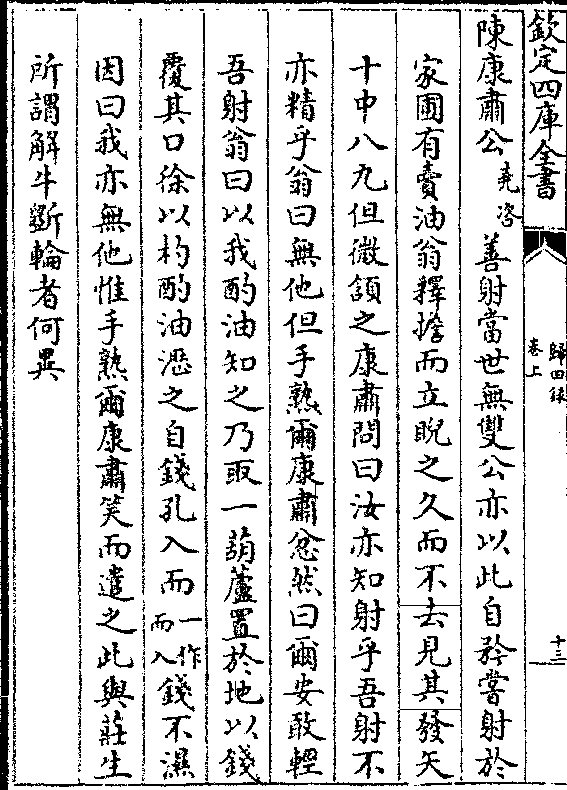
\includegraphics[height=0.65\textwidth]{Figures/Sale_Oil_Ouyang.png}
%\hspace{1pt}
%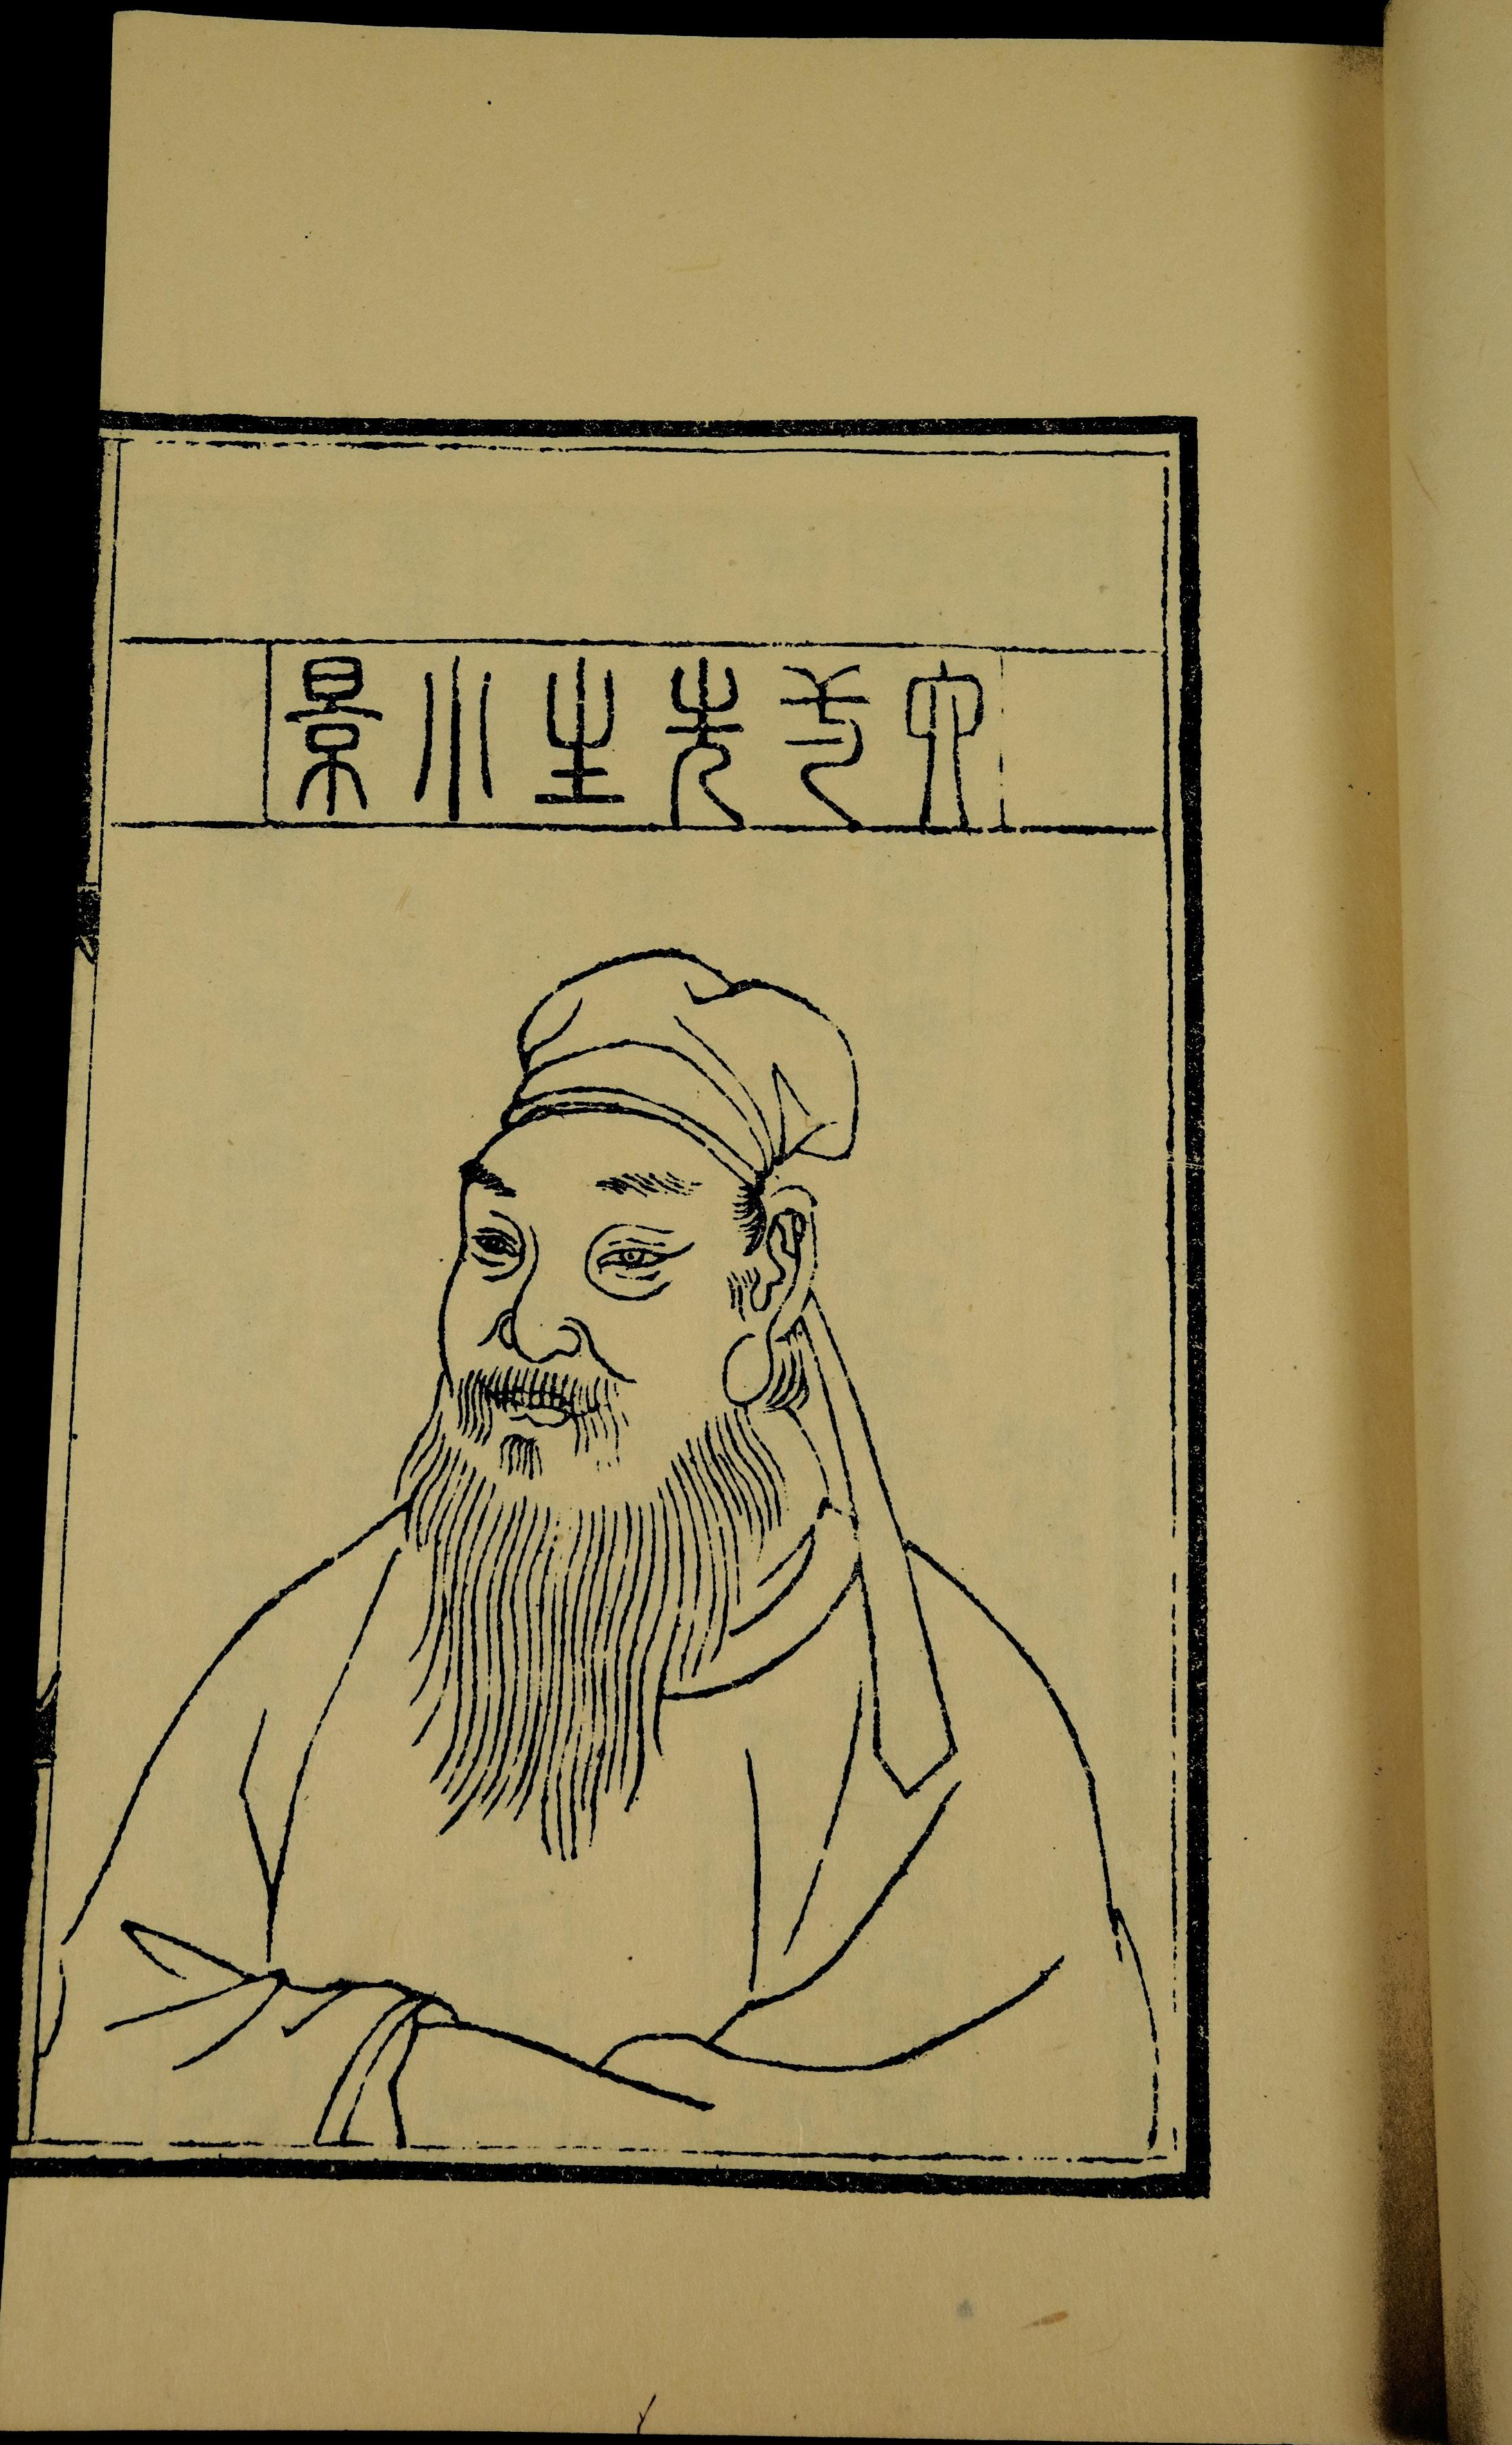
\includegraphics[height=0.65\textwidth]{Figures/Ouyang_Xiu-2.jpg}
%\caption{\fontsize{6.2pt}{5.2pt}\selectfont{欧阳修(1007-1072)~《欧阳文忠公文集$\cdot$归田录》~卷上}}
%\label{Sale_oil}
%\end{figure}
%}
